\section{Homotopy and Cauchy's Theorem}

\begin{definition}
    Let $\y_0:[0,1] \xrightarrow{} G$ and $\y_1:[0,1] \xrightarrow{} G$ be
    paths (not necesarily closed, nor rectifiable) on a region $G$. We say that
    $\y_0$ is \textbf{homotopic}
    to $\y_1$ in $G$ if there exists a continuous complex valued function
    $\Gamma:[0,1] \times [0,1] \xrightarrow{} G$ such that
    \begin{equation*}
        \Gamma(s,0)=\y_0(s) \text{ and } \Gamma(s,1)=\y_1(s) \text{ for all } 0
        \leq s \leq 1
    \end{equation*}
    We call $\Gamma$ a  \textbf{homotopy} between $\y_0$ and $\y_1$, and write
    $\Gamma:\y_0 \sim \y_1$; or simply $\y_0 \sim \y_1$.
\end{definition}

\begin{lemma}\label{4.6.1}
    Homotopy between paths is an equivalence relation.
\end{lemma}
\begin{proof}
    Let $G$ be a region. For any path $\y$, the identity function $I:[0,1] \times
    [0,1]  \xrightarrow{} G$ defined by  $I(s,t)=\y(s)$ for all $0 \leq s, \leq 1$
    defines a homotopy between $\y$ and itself.

    Now, let $\y_0$ and $\y_1$ be paths, and suppose that $\Gamma:\y_0 \sim \y_1$.
    Let $\Lambda:[0,1] \times [0,1] \xrightarrow{} G$ be defined by
    \begin{equation*}
        \Lambda(s,t)=\Gamma(s,1-t)
    \end{equation*}
    Then we have that $\Lambda(s,0)=\y_1(s)$, $\Lambda(s,1)=\y_0(s)$. Moreover,
    since $\Gamma$ is continuous, so is $\Lambda$. Hence  $\Lambda: \y_1 \sim \y_0$.

    Now, suppose that for paths $\y_0$, $\y_1$, and $\y_2$, that $\Gamma: \y_0
    \sim \y_1$, and $\Lambda:\y_1 \sim \y_2$. Define then $\Phi:[0,1] \times [0,1]
    \xrightarrow{} G$ by
    \begin{equation*}
        \Phi(s,t)=\begin{cases}
            \Gamma(s,2t), \text{ if } 0 \leq t \leq \frac{1}{2} \\
            \Lambda(s,2t-1), \text{ if } \frac{1}{2} \leq t \leq 1
        \end{cases}
    \end{equation*}
    By the pasting lemma from topology, we get that $\Phi$ is continuous.
    Moreover, we have $\Phi(s,0)=\Gamma(s,0)=\y_0$, and
    $\Phi(s,1)=\Lambda(s,1)=\y_2$. Therefore  $\Phi: \y_0 \sim \y_2$.
\end{proof}
\begin{corollary}
    If $\y_0$ and $\y_1$ are closed paths homotopic to each other via a homotopy
    $\Gamma$, then  $\Gamma(0,t)=\Gamma(1,t)$ for all $0 \leq t \leq 1$.
\end{corollary}

\begin{figure}[h]
    \centering
    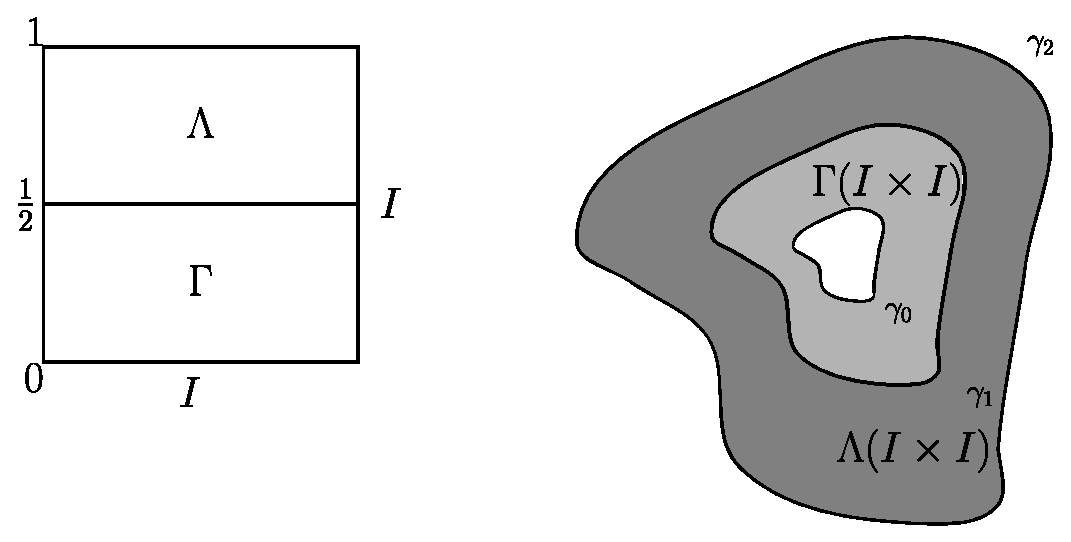
\includegraphics[scale=0.5]{Figures/Chapter4/homotopy.eps}
    \caption{The transitivity of homotopy between the paths $\y_0$, $\y_1$, and
    $\y_2$.}
    \label{figure_4.3}
\end{figure}

\begin{definition}
    We call a region $G$ of  $\C$  \textbf{convex} if for any two points $a,b
    \in G$, then line segment  $[a,b] \subseteq G$. We call $G$  \textbf{star
    shaped} if there exists a point $a \in G$ such that for any  $z \in G$, the
    line segment $[a,z] \subseteq G$.
\end{definition}

\begin{lemma}\label{4.6.2}
    Let $G$ be a star shaped region. If  $\y_0$ is homotopic to a constant curve
    defined by some  $a \in G$, then every closed rectifiable curve is homotopic
    to  $\y_0$.
\end{lemma}
\begin{proof}
    Let $a \in G$, and suppose without loss of generality that  $\y_0$ is the
    constant curve defined by $a$; i.e.  $\y_0(s)=a$ for all $0 \leq s \leq 1$.
    Let  $\y_1$ be a closed rectifiable path in $G$, and take $\Gamma:[0,1]
    \times [0,1] \xrightarrow{} G$ defined by
    \begin{equation*}
        \Gamma(s,t)=t\y_1(s)+(1-t)\y_0
    \end{equation*}
    since $G$ is star shaped; in particular, about  $a$, we see that  $\Gamma:
    \y_1 \simn \y_0$.
\end{proof}

\begin{definition}
    We call a closed rectifiable path $\y$ in a region $G$
    \textbf{nullhomotopic} if it is homotopic to a constant curve in $G$. We
    write  $\y \sim 0$.
\end{definition}

\begin{theorem}\label{4.6.3}
    If $\y_0$ and $\y_1$ are closed rectifiable curves in a region $G$, and $f$
    is a function analytic on $G$, then
    \begin{equation*}
    \int_{\y_0}{f}=\int_{\y_1}{f}
    \end{equation*}
\end{theorem}
\begin{proof}
    Let $I=[0,1]$ and $\Gamma:I \times I \xrightarrow{} G$ a homotopy between
    $\y_0$ and $\y_1$. Then since $\Gamma$ is continuous, and  $I \times I$ is
    compact,  $\Gamma$ is uniformly continuous, and  $F(I \times I) \subseteq G$
    is also compact. Thus
    \begin{equation*}
        r=d(\Gamma(I \times I), \com{\C}{G})>0
    \end{equation*}
    and there exists an $n \in \Z^+$ such that if
    \begin{equation*}
        (s-s')^2+(t-t')^2<\frac{4}{n^2}
    \end{equation*}
    then
    \begin{equation*}
        |\Gamma(s,t)-\Gamma(s',t')|<r
    \end{equation*}

    Now, let $Z_{j,k}=\Gamma(\frac{j}{n},\frac{k}{n})$, for all $0 \leq j,k \leq
    n$, and put  $J_{j,k}=[\frac{j}{n},\frac{j+1}{n}] \times
    [\frac{k}{n},\frac{k+1}{n}]$ for all $0 \leq j,k \leq n-1$. Then
    $\diam{J_{j,k}}=\frac{\sqrt{2}}{n}$  and $\Gamma(J_{j,k}) \subseteq
    B(Z_{j,k},r)$

    \begin{figure}[h]
        \centering
        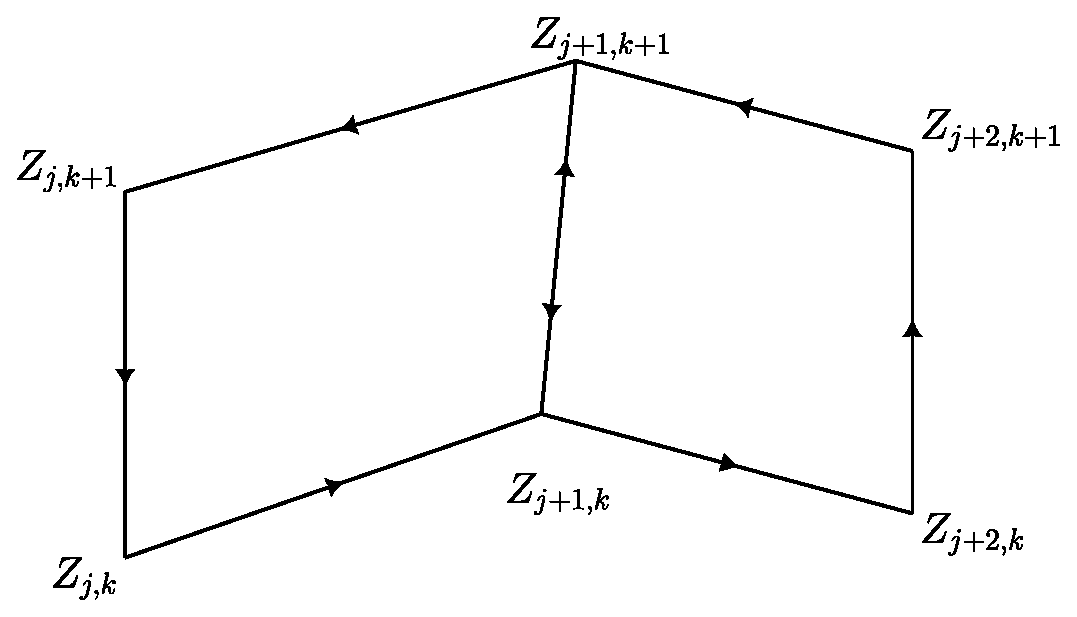
\includegraphics[scale=0.5]{Figures/Chapter4/cauchy_2.eps}
        \caption{The polygon $P_{j,k}$.}
        \label{figure_4.4}
    \end{figure}

    Now, letting $P_{j,k}=[Z_{j,k}, Z_{j+1,k}, Z_{j+2,k}, Z_{j+2,k+1},
    Z_{j+1,k+1}, Z_{j,k+1}, Z_{j,k}]$ a closed polygon described in figure
    \ref{figure_4.4}, sicne open balls are convex, we have  $P_{j,k} \subseteq
    B(Z_{j,k},r)$. However, also notice that if $f$ is any function analytic on
     $G$, then
     \begin{equation*}
         \int_{P_{j,k}}{f}=0
     \end{equation*}

     Now, let $Q_k=[Z_{0,k}, \dots, Z_{n,k}]$ a closed polygon, observe that for
     any function $f$ analytic on $G$, we have
     \begin{equation*}
         \int_{\y_0}{f}=\int_{Q_0}{f}
     \end{equation*}
     Indeed, let $\s_j(s)=\y_0(s)$ for all $\frac{j}{n} \leq s \leq
     \frac{j+1}{n}$. Then the path $\s_j+[Z_{j+1,0},Z_{j,0}]$ is a closed
     rectifiable path in the open ball $B(Z_{j,0},r) \subseteq G$. Hence we get
     \begin{equation*}
         \int_{\s_j}{f}=-\int_{[Z_{j+1,0},Z_{j,0}]}{f}=
         \int_{[Z_{j,0},Z_{j+1,0}]}{f}
     \end{equation*}
     Then adding both sides of this equation for $0 \leq j \leq n$ gives us the
     above assertion. By similar reasoning, we also find that
     \begin{equation*}
         \int_{\y_1}{f}=\int_{Q_n}{f}
     \end{equation*}
     for any $f$ analytic on $G$.

     Now, since $\int_{P_{j,k}}{f}=0$ for the polygon $P_{j,k}$, we get that
     \begin{equation*}
         \sum_{j=0}^{n-1}{\int_{P_{j,k}}{f}}=0
     \end{equation*}
     Notice now, that $\int_{P_{j,k}}{f}$ includes the integral over the line
     segment $[Z_{j+1,k}, Z_{j+1,k+1}]$, which is also the integral over the
     line segment $[Z_{j+1,k+1}, Z_{j+1,k}]$, which is part of the integral
     $\int_{P_{j+1,k}}{f}$. Moreover, since
     $Z_{0,k}=\Gamma(0,\frac{k}{n})=\Gamma(1,\frac{k}{n})=Z_{n,k}$ we get
     \begin{equation*}
         [Z_{o,k+1},Z_{0,k}]=-[Z_{1,k},Z_{1,k+1}]
     \end{equation*}
     Then cancelling out the terms in the expansion leaves us with
     \begin{equation*}
         \int_{Q_k}{f}=\int_{Q_{k+1}}{f}
     \end{equation*}
     Therefore, by transitiviy, we have proven what is required.
\end{proof}
\begin{corollary}
    If $\y$ is a closed rectifiable path, nullhomotopic on a region  $G$, then
    \begin{equation*}
        W(\y,z)=0 \text{ for all } z \in \com{\C}{G}
    \end{equation*}
\end{corollary}

\begin{theorem}[Cauchy's Theorem]\label{4.6.4}
    IF $f:G \xrightarrow{} \C$ is a function analytic on a region $G$, and  $\y$
    is a nullhomotopic, closed rectifiable path in $G$, then
    \begin{equation*}
        \int_\y{f}=0
    \end{equation*}
\end{theorem}
\begin{proof}
    This theorem follows from the above. Let $\y \sim y_0$ where $\y_0(s)=a$ for
    all $0 \leq s \leq 1$, and some  $a \in G$. Then notice that  $W(\y_0,z)=0$
    for all $z \in \com{\C}{G}$, so by Cauchy's integral formula
    \begin{equation*}
        \int_{\y_0}{f}=0
    \end{equation*}
    Then the homotopy gives us the required integral.
\end{proof}

\begin{definition}
    Let $\y_0:[0,1] \xrightarrow{} G$ and $\y_1:[0,1] \xrightarrow{} G$ be
    paths (not necesarily closed, nor rectifiable) in a region $G$, such that
    their endpoints coincide; i.e.  $\y_0(0)=\y_1(0)=a$ and $\y_0(1)=\y_1(1)=b$.
    Then we call $\y_0$ \textbf{fixed end point homotopic} to $\y_1$ if there
    exists a continuous function $\Gamma:[0,1] \times [0,1] \xrightarrow{} G$
    such that $\Gamma$ defines a homotopy between  $\y_0$ and $\y_1$, and
    \begin{equation*}
        \Gamma(0,t)=a \text{ and } \Gamma(1,t)=b \text{ for all } 0 \leq t \leq
        1
    \end{equation*}
\end{definition}

\begin{lemma}\label{4.6.5}
    Fixed endpoint homotopy between paths is an equivalence relation.
\end{lemma}
\begin{proof}
    The proof is identical to that of lemma \ref{4.6.1}.
\end{proof}

\begin{theorem}[The Path Independence Theorem]\label{4.6.6}
    If $\y_0$ and $\y_1$ are rectifiable paths from $a$ to $b$, fixed endpoint
    homotopic in a region $G$, then for any function $f$ analytic on $G$
    \begin{equation*}
        \int_{\y_0}{f}=\int_{\y_1}{f}
    \end{equation*}
\end{theorem}
\begin{proof}
    Since $\y_0$ and $\y_1$ are rectifiable with $\y_0(0)=\y_1(0)=a$ and
    $\y_0(1)=\y_1(1)=b$,  then the path $\y_0-\y_1$ taken by going along $\y_0$
    and the along the reverse of $\y_1$ is a closed rectifiable path. Now, let
    $\Gamma:\y_0 \sim \y_1$ a fixed point homotopy between $\y_0$ and $\y_1$.
    Define $\y:[0,1] \xrightarrow{} G$ by
    \begin{equation*}
        \y(s)=\begin{cases}
            \y_0(3s), \text{ if } 0 \leq s \leq \frac{1}{3} \\
            b, \text{ if } \frac{1}{3} \leq s \leq \frac{2}{3}  \\
            \y_1(3-3s), \text{ if } \frac{2}{3} \leq s \leq 1   \\
        \end{cases}
    \end{equation*}
    Then define $\Lambda:[0,1] \times [0,1] \xrightarrow{} G$ by
    \begin{equation*}
        \Lambda(s,t)=\begin{cases}
            \Gamma(3s(1-t),t), \text{ if } 0 \leq s \leq \frac{1}{3} \\
            \Gamma(1-t, 3s-1+2t-3st), \text{ if } \frac{1}{3} \leq s \leq \frac{2}{3}  \\
            \y_1((3-3s)(1-t)), \text{ if } \frac{2}{3} \leq s \leq 1   \\
        \end{cases}
    \end{equation*}
    Then $\Lambda:\y \sim 0$, which makes  $\y$ null homotopic. Therefore, by
    Cauchy's theorem
    \begin{equation*}
        \int_{y}{f}=\int_{\y_0}{f}-\int_{\y_1}{f}=0
    \end{equation*}
\end{proof}

\begin{definition}
    We call a region $G$ of  $\C$  \textbf{simply connected} if every closed
    path in $G$ is nullhomotopic.
\end{definition}

\begin{theorem}\label{4.6.7}
    If $G$ is simply conneced in  $\C$, and  $f$ is analytic on $G$, then for
    any closed rectifiable path $\y$ in  $G$
    \begin{equation*}
        \int_\y{f}=0
    \end{equation*}
\end{theorem}
\begin{proof}
    This follows directly from the definition of simple connectedness and
    Cauchy's theorem.
\end{proof}
\begin{corollary}
    If $G$ is simply connected and  $f:G \xrightarrow{} \C$ is holomorphic on $G$,
    then  $f$ has a primitive.
\end{corollary}
\begin{proof}
    Fix $a \in G$, and take  $\y_0,\y_1$ and two rectifiable paths from $a$ to a
    point  $z \in G$. Then we get from theorem \ref{4.6.6}
    \begin{equation*}
        \int_{\y_0-\y_1}{f}=\int_{\y_0}-\int_{\y_1}{f}=0
    \end{equation*}
    where $\y_0-\y_1$ is the closed rectifiable path from $a$ to  $a$ taken
    along first $\y_0$ and then the revers of $\y_1$. Hence we obtain a well
    defined complex valued function $F:G \xrightarrow{} \C$ by taking
    \begin{equation*}
        F(z)=\int_\y{f(z) \ dz}
    \end{equation*}
    where $\y$ is any rectifiable curve from $a$ to $z$.

    Now, take  $z_0 \in G$, and $r>0$ such that $B(z_0,r) \subseteq G$, and let
    $\y$ be a rectifiable path from  $a$ to $z_0$. Then for $z \in B(z_0,r)$,
    define $\y_2=\y+[z_0,z]$, the path defined by going along $\y$, and then the
    line segment $[z_0,z]$. Then we have
    \begin{equation*}
        \frac{F(z)-F(z_0)}{z-z_0}=\frac{1}{z-z_0}\int_{[z_0,z]}{f}
    \end{equation*}
    Then
    \begin{equation*}
        \frac{F(z)-F(z_0)}{z-z_0}-f(z_0)=\frac{1}{z-z_0}\int_{[z_0,z]}{f(w)-f(z_0)
        \ dw}
    \end{equation*}
        taking abosulte values gives us
    \begin{equation*}
        \Big{|}\frac{F(z)-F(w_0)}{z-w_0}-f(w_0)\Big{|} \leq
        \sup_{w \in [w_0,z]}{\{|f(w)-f(w_0)|\}}
    \end{equation*}
    so that
    \begin{equation*}
        \lim_{z \xrightarrow{} w_0}{\frac{F(z)-F(w_0)}{z-w_0}}=f(w_0)
    \end{equation*}
    which gives $F'(z_0)=f(z_0)$.
\end{proof}
\begin{corollary}
    Let $G$ be a simply connected region, and  $f:G \xrightarrow{} \C$ a
    function holomorphic on $G$ such that  $f(z) \neq 0$ for al $z \in G$. Then
    there exists a function  $g:G \xrightarrow{} \C$, holomorphic on $G$ such that
    \begin{equation*}
        f(z)=\exp{g(z)}
    \end{equation*}
    In particular, if $z_0,w_0 \in G$, and $\exp{w_0}=f(z_0)$, we can choose $g$
    such that $g(z_0)=w_0$.
\end{corollary}
\begin{proof}
    By hypothesis, we get that since $f$ never vanishes, the function
    $\frac{f'}{f}$ is holomorphic on $G$, and hence has a primitive $g_1$. Now, if
    $h(z)=\exp{g_1(z)}$, then $h$ is holomorphic on  $G$, and never vanishes. Thus
     $\frac{f}{h}$ is holomorphic on $G$ and has derivative
     \begin{equation*}
         \frac{hf'-fh'}{h^2}
     \end{equation*}
     but $h'=g_1'h$, so that $hf'-fh'=0$. This makes  $\frac{f}{h}$ constant on
     $G$. That is
     \begin{equation*}
         f(z)=c\exp{g_1(z)} \text{ for some } c
     \end{equation*}
     Moreover, since $\exp$ is periodic, for som  $c'$ we also have
     \begin{equation*}
         f(z)=c\exp{(g_1(z)+c')}
     \end{equation*}
     Choose then $g(z)=g_1(z)+c'+2i\pi{k}$, where $k \in \Z$. This gives us the
     required $g$.
\end{proof}

\begin{definition}
    Let $G$ be open in $\C$. We call a closed path $\y$ in $G$
    \textbf{nullhomologous} if
    \begin{equation*}
        W(\y,z)=0 \text{ for all } z \in \com{\C}{G}
    \end{equation*}
    We write
    $\y \approx 0$.
\end{definition}
